\chapter{Classifier Trees}

Classifiers described in this paper return results in form of a class label that provided pattern was classified to. Such approach leaves no room for estimating class-belonging probabilities which, in return, results in inability to reject provided data. By combining those classifiers and organising them in a complex structures it is possible to create objects with unique rejection capabilities in exchange for slightly increased pattern-processing time. This chapter describes classifier structures in form of binary trees.

\section{Balanced Tree}

\subsection{Description}

Balanced Tree structure utilises clustering algorithms for its creation. It is usually shaped as a balanced binary tree, thus the name, with classifier in each of its nodes. Each node represents a set of classes that are currently taken into consideration as native ones for provided pattern. By traversing down the tree certain classes get rejected and the pattern is moved forward to the next node that represents only remaining classes. Decision as to which classes should be put in each of the child nodes is made by clustering algorithm that divides set of remaining classes from parent node into two and assigns each part for each child node. If there's only one remaining class, tree leaf is created instead. Each node, except for leafs, contains binary classifier trained on data that is based on clustering algorithm results. What it mean is that patterns from training data set, that belong to classes dedicated for left child node, are joined together and are treated as one big class '0'. The same goes for patterns that belong to the right child node, except for the class number which is '1'. By having two, new data sets that represent two different classes, the parent node can finally create binary classifier. During classification procedure, after receiving new, unknown pattern each node uses its classifier to assign either '0' or '1' label to this pattern, which is then used to send it to left or right child accordingly for further classification. Balanced Tree leafs also utilize their classifiers but those are created in a different way. Because of the fact that each leaf represents one class, and has no children there's no way to create data set for classifier using algorithm for non-leaf node. To overcome this problem each leaf is treated as a node with left child representing the same class as the leaf, and the right child representing all remaining classes. That way classifier is trained on two-class data and can be viewed as 'one-vs-rest' classifier. When it comes to classifying new, unknown pattern leaf uses its classifier to determine pattern's label. In case of '0' (meaning it should be sent to left child) the pattern is treated as an element from class represented by leaf. If the resulting label is '1' the pattern gets rejected and treated as a foreign one.

\subsection{Implementation details}

Creation of Balanced Tree structure starts from tree root and is done recursively. Each node, that is not a tree leaf, is assigned certain set of classes which is a subset of all classes in a tree (root node is assigned all). The next step involves clustering method dividing node's class set into two disjoint sets. This procedure is done on 'class central points' which are average points of all elements in each class. Clustering algorithm divides those points thus providing two new sets for both child nodes. After that node trains its classifier on data set consisting of two classes created by taking all elements from training data for left and right child nodes' classes sets. The node-creation procedure is then applied for both node's children. The leaf creation algorithm is slightly different as it does not need usage of clustering. Classifier is trained on data set created from combining elements from training data that belongs to the same class the leaf node represents (those points' new class is labelled '0') and elements from every other class (which are labelled '1')\label{balanced_tree:one-vs-rest}. To ensure that both '0' and '1' classes have the same number of entries the '1' class set must be trimmed. This is done at its creation step by taking less elements from each class in order to have the same number (or nearly identical) of elements overall in the whole set, e.g. having training data set consisting of ten classes labelled from '0' to '9', with total of 10,000 elements, set '0' for leaf representing class '2' will have 1,000 entries of elements from class '2' taken from training data and set '1' will have 999 elements in total but will consist of elements from classes '0', '1', '3', '4', '5', '6', '7', '8', '9' taken from training data with 111 elements from each class.

\begin{figure}[!t]
	\centering
	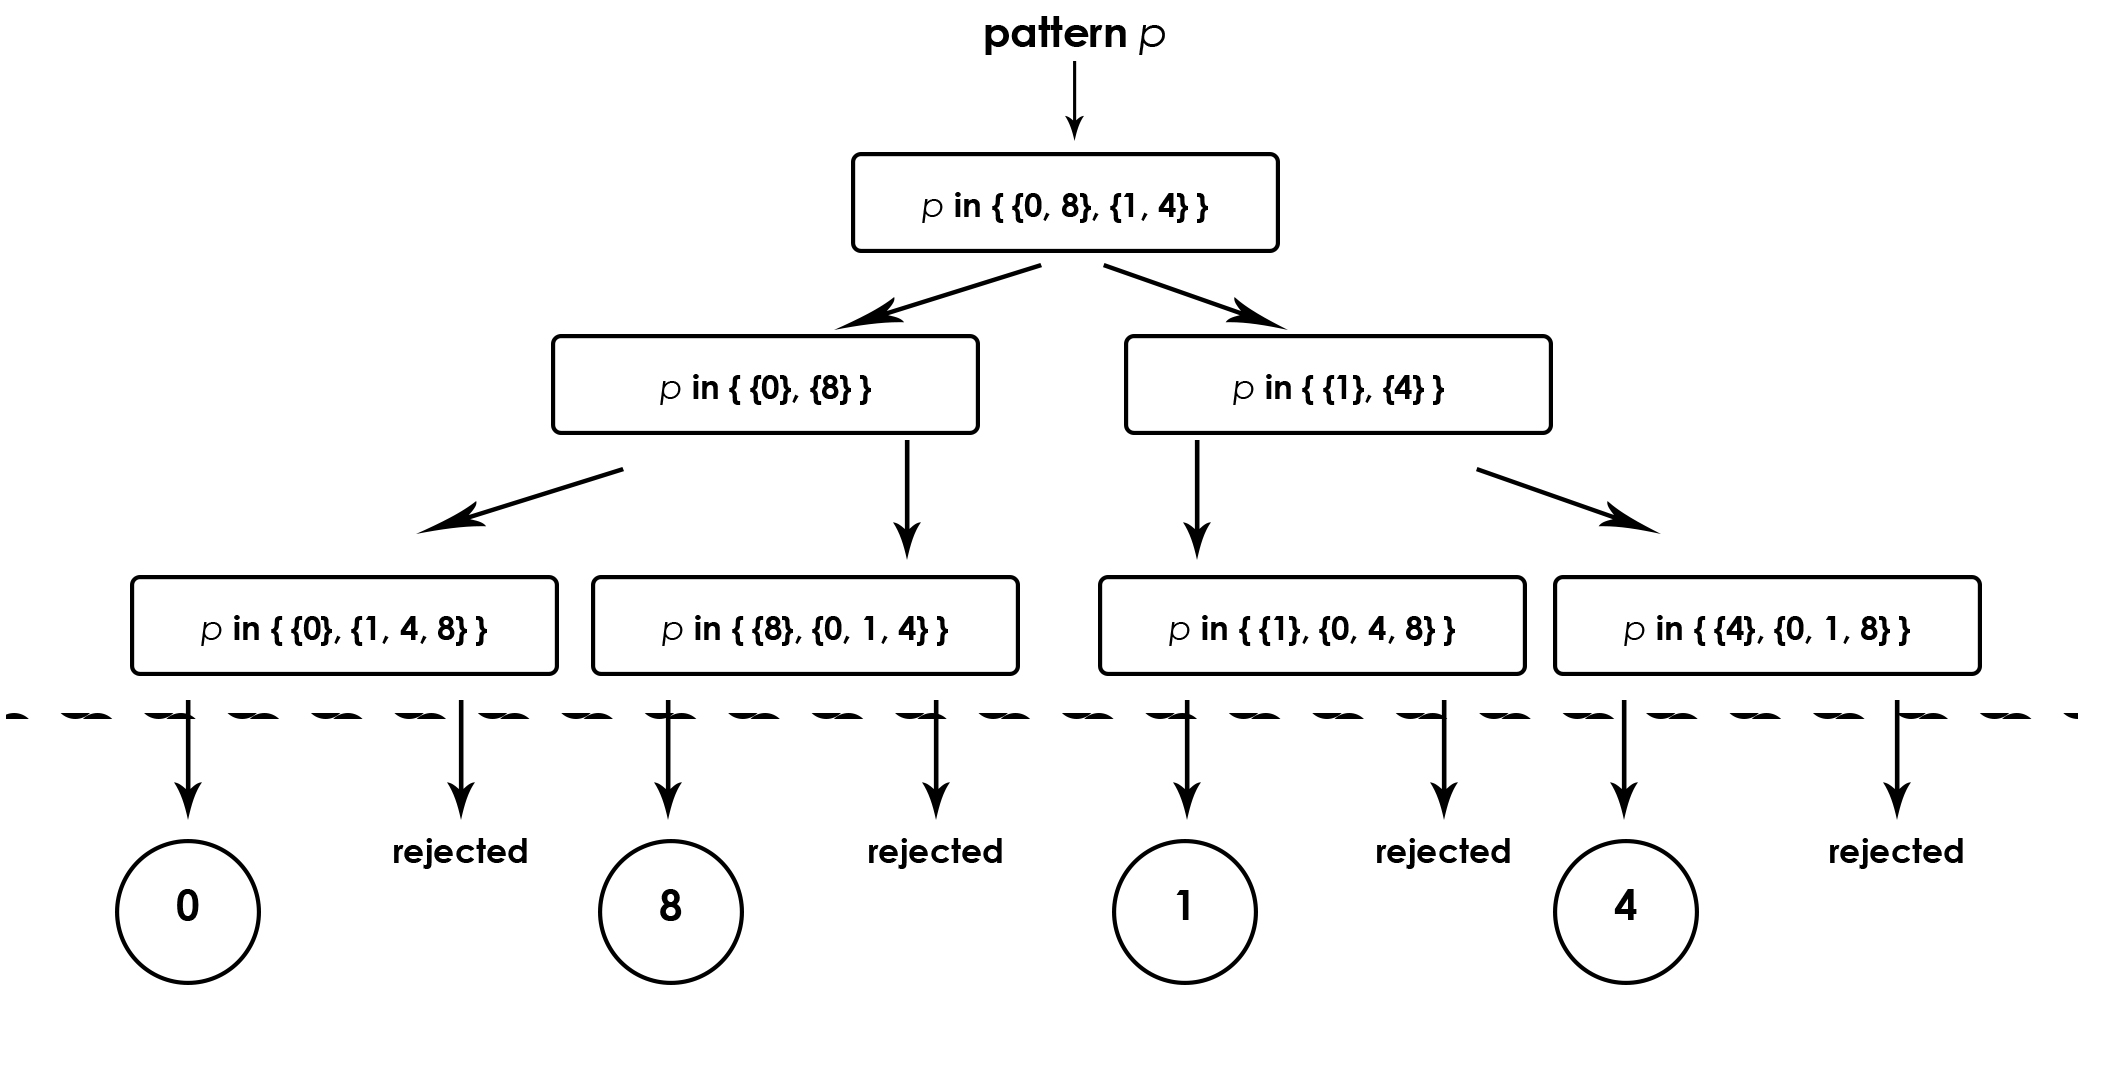
\includegraphics[width=1\textwidth]{Figures/balanced_tree.jpg}
	\caption{Balanced Tree example, trained on samples with class lables 0, 1, 4, 8. Each node (depicted as rounded rectangle) holds classifier that decides if provided pattern p is more similar to elements in the left or right child (p in \{\{left\_child\_classes\}, \{rigt\_child\_classes\}\}). Dotted line at the bottom of the image depicts final decisions (element classified as a member of certain class or rejected).}
	\label{fig:rejection_version1}\vspace{-3pt}
\end{figure}

\section{Slanting Tree}

\subsection{Description}

Slanting Tree structure has its nodes chained in a very specific way. It always has $ 2n $ nodes (including leafs) where $n$ is the number of classes in the training set. Each node represents only one class, there are two nodes per class in total, one non-leaf node and one tree leaf. Non-leaf nodes play role of initial filters that try to conclude if the received unknown pattern belongs to a class this particular node represents. In case of classifying such pattern as a native one further classification is done by a child leaf node representing the same native class. If the leaf node also classifies received element as a native one no further classification is done and the pattern is marked as an object from leaf's class. If the opposite situation occurs and the element is not recognized, it is sent to the next non-leaf node in the tree as if the leaf's parent node did not recognize the element either. In case of no more nodes in the tree left the unknown pattern is rejected and treated as a foreign one.

\subsection{Implementation details}

Creation of Slanting Tree is done recursively, starting from the root node. All classes that should be distinguishable by this tree structure are sorted by their labels and stored in an array object. This object is later used during node creation method to check what classes have already been covered by previous nodes. Every non-leaf node represents only one native class and has its binary classifier trained in 'one-vs-rest' manner, the same way the tree leafs' classifiers in Balanced Tree are (see \ref{balanced_tree:one-vs-rest}). The next step involves creating left child node for the next native class in the array object that has not yet been used. In case of no classes left the function returns without creating new node. The last step consists of right child creation, which is a leaf node. Leafs in a Slanting Tree represent the same native classes their parent node did, but their classifiers, although built using same 'one-vs-rest' approach, are trained on a different data sets in order to create more accurate results. Usually trained classifier does not achieve 100\% accuracy even on a training test that was used during its creation. There are some samples from first class that get classified as elements from the second and vice versa. Such mistakes can help determine what kind of corrections can be made to the classifier. For every non-leaf node, after its classifier training, there's set of elements from the first class that were correctly recognized (those are the elements from the class this particular node is representing) and set of elements from the second class that were mistakenly recognized as elements from the first class. Those two sets are used in this node's child leaf node's classifier creation. Of course before training those two sets must be the same size, ideally having the same number of elements as two sets used in parent's classifier training. For each missing element in either of sets the new object is generated by randomly selecting one element from this set and applying normal distribution (with standard deviation 1) to all of its features in a feature vector, thus getting new sample that can be added to the set. In case of having less than certain number of elements (implementation checks for 10 or less elements) in either of sets before new point generation algorithm takes place, those sets are filled with randomly selected points from parent node's classifier training sets.
